\section{Operating principles}

Having successfully constructed the DNA nanopiston, the operation cycle, presented in
Figure \ref{fig:operating}a, can now be discussed. For convenience, we take the
rotaxane-ds configuration as the starting
point of this cycle. Here the suffix ’ds’ alludes to the predominantly dsDNA composition
of this rotaxane configuration. The power stroke of the molecular machine is initiated by
bringing the appropriate chemical fuel, ssDNA $4$ $(0.5\ \mu M)$, into solution at the
trans-side.
The DNA strand is fully complementary to ssDNA $2$, thereby inducing a strand
displacement. Here the flexible overhang located at the end of ssDNA $2$ is used to
mediate the hybridisation of ssDNA $2$ and $4$. In Figure \ref{fig:operating}a the
transition is shown, going from state $(1)$ to $(3)$ the blue strand is removed from
rotaxane-ds.

During the strand displacement reaction, it is hypothesised that different transient
states can possibly occur. One of the possible scenario's describes the hybridisation
happening inside of the nanopore. This scenario is deemed to be unlikely, since this
process would require three strands of ssDNA to be simultaneously present inside the
constriction of the nanopore. Alternatively, the hybridisation can take place outside of
the nanopore, in the trans-side of the reservoir. This process implies that the
neutravidin protein would enter the lumen of the pore, which has been showed to be
possible by previous studies. \cite{Lu2018} This variation of the transient state is
thereby thought to be the most probable.

The resulting configuration is called the rotaxane-ss in view of the fact that it is
predominately composed of ssDNA, seen in state (3). During this process a DNA duplex,
composed of
the ssDNA 2 and 4, is released into the trans-side of the reservoir.

Subsequently the cargo strand, $0.5\ \mu M$ of ssDNA $2$,  is brought into solution at
the cis-side, inducing the piston's recovery stroke. In this process the cargo hybridises
with the rotaxane-ss, re-establishing a rotaxane-ds structure and completing the cycle,
seen in the transition from state $(3)$ back to $(1)$.
Each piston iteration transports one cargo strand, from the cis- to the trans-side of
the nanopore, turning over one fuel strand in the process.

Important to note is that no external potential is specified for operating the DNA
nanopiston. In contrast to earlier DNA transporters, the piston is able to function in a
range of applied transmembrane biases. Experimentally, it is verified that the
cycle operates at positive, $+20\ mV$, $+50\ mV$ and $+100\ mV$ and negative, $ - 20\
mV$. The limited range observed for negative voltages is most likely resulting from the
inability of the fuel strand to hybridise with the toehold of rotaxane-ds. This
hybridisation reaction is a rate limiting process, resulting in faster cycles at positive
then at negative applied bias, shown in Figure \ref{fig:operating}b. Other factors, like
the accessibility of cargo strands during the hybridisation of rotaxane-ss also influence
the cycle rate.

The ability of the nanopiston to transport cargo both with and against an external bias
is an important property of this molecular machine. It suggests that the externally
applied bias might not be necessary for its functioning. Suspected is that the entropic
interactions between the DNA strands and the nanopore are expected to play an important
role in this behaviour. To accurately understand these effects, further analysis is
needed.

\vspace{1cm}
\begin{figure}[ht!]
  \begin{centering}
  \adjustbox{minipage=1.3em,valign=t}{\subcaption{}\label{sfig:testb}}%
  \begin{subfigure}[t]{\dimexpr\linewidth-1.3em\relax}
  \centering
  \hspace{-3.5cm}
  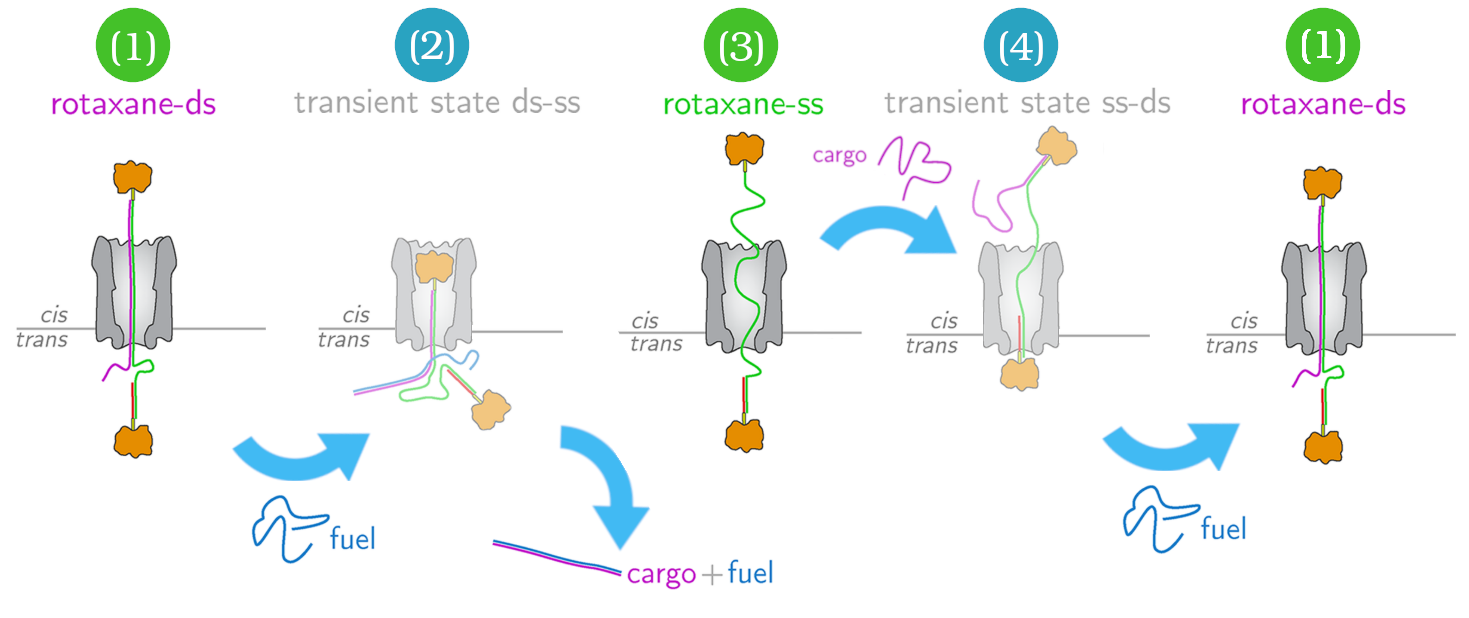
\includegraphics[width=0.8\linewidth,valign=t]{Figures/cycle.png}
  \end{subfigure}
  \vspace{0.6cm}
  \adjustbox{minipage=1.3em,valign=t}{\subcaption{}\label{sfig:testa}}%
  \begin{subfigure}[t]{\dimexpr\linewidth-1.3em\relax}
  \centering
  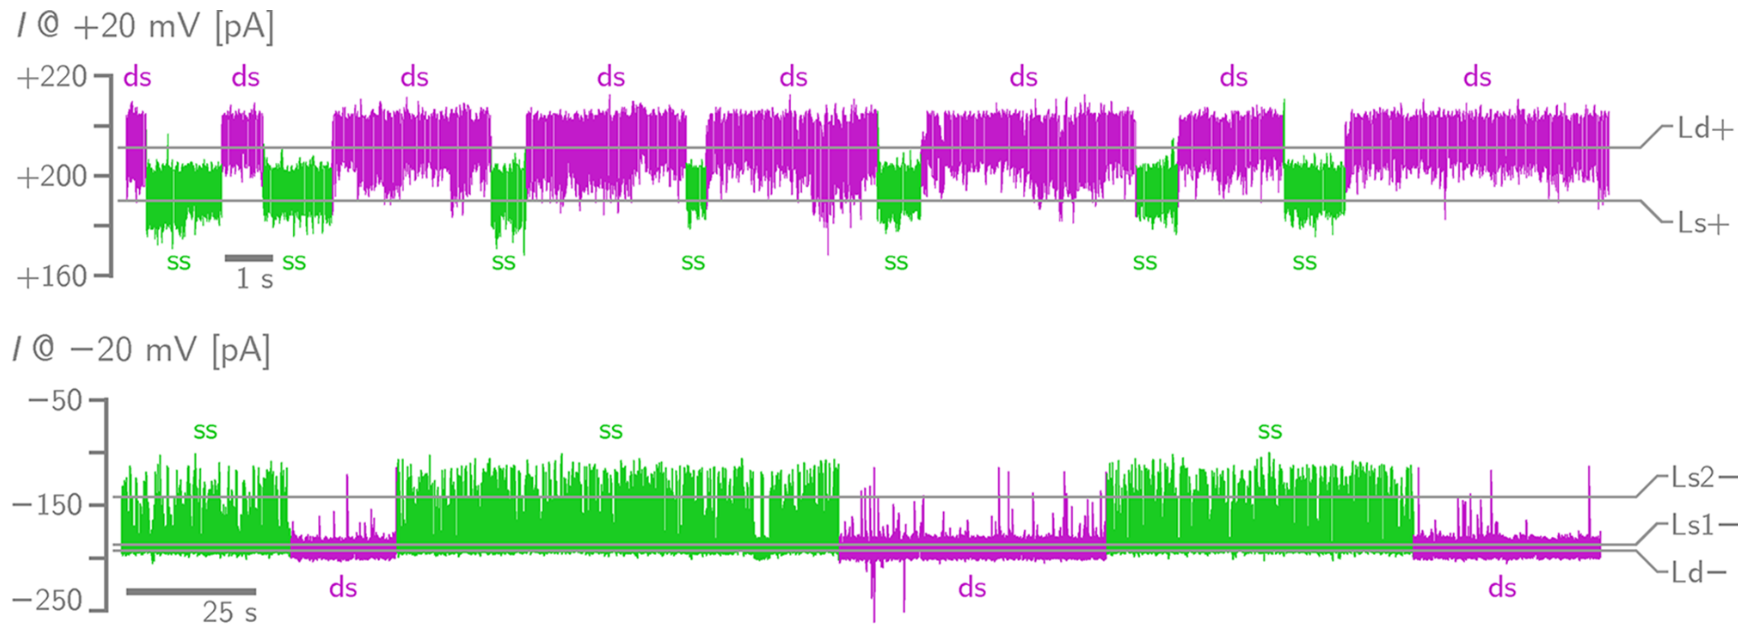
\includegraphics[width=\linewidth,valign=t]{Figures/FluctuationRotaxane.png}
  \end{subfigure}%
  \end{centering}
  \caption[Illustration of the DNA nanopiston cycles.]{\linespread{0.3}{\small (a)
       Illustration of the DNA nanopiston cycles. Here the stable states of the piston
       operation are indicated with green labels and the short-lived transient states
       with magenta labels. The cycle is facilitated by the fuel and cargo strand present
       in the trans- and cis-reservoirs. (b) Time traces of the current measured
       during the nanopiston cycle.  The rotaxane-ds conformation is shown in purple and
   the rotaxane-ss conformation is shown in green. The horizontal lines mark the average
   measured currents in rotaxane-ds and rotaxane-ss, indicated with Ld and Ls,
   respectively. Figures adapted from reference \cite{Bayoumi21}.}}
\label{fig:operating}
\end{figure}
